\subsection{Platform Initialization \gls{pi} Boot Sequence}
Platform Initialization \gls{pi} compliant system firmware has to support the six phases: 
\begin{enumerate}
	\item Security (\gls{sec}) Phase
	\item Pre-efi Initialization (\gls{pei}) Phase
	\item Driver Execution Environment (\gls{dxe}) Phase
	\item Boot device selection (\gls{bds}) Phase
	\item Run time (RT) services and After Life (AL) (transition from the OS back to the firmware) of system. 
\end{enumerate}
Figure \ref{fig:design-pi-boot-phases} describes the phases and transition in detail.

\begin{figure}[h]
	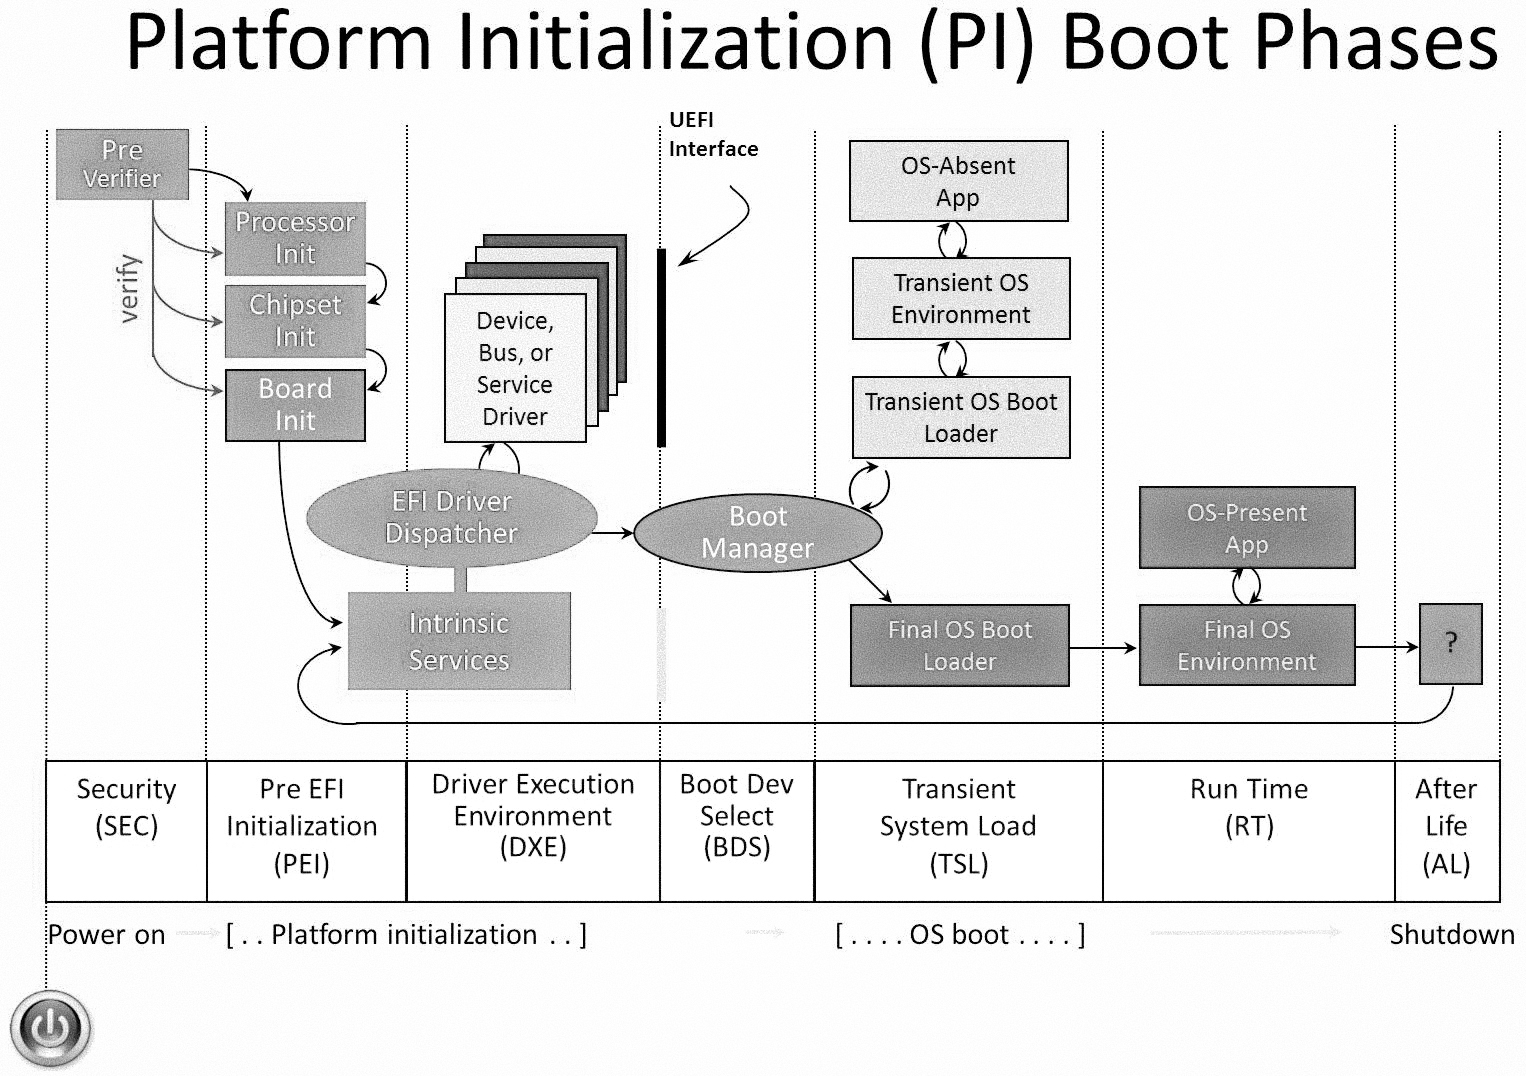
\includegraphics[width=\linewidth]{PI_Boot_Phases}
	\caption{\gls{pi} Boot Phases}\label{fig:design-pi-boot-phases}
\end{figure}

\subsection{Security (\gls{sec})}
The Security (SEC) phase is the initial phase in the PI Architecture and is liable for the following:
\begin{itemize}
	\item Handling restart events of all platform
	\item Creation of a temporary memory store
	\item Bringing the root of trust in the system
	\item Transit handoff information to next phase - the PEI Foundation
\end{itemize}
The security section may have the modules with source code scripted in assembly language. Hence, some \gls{edk2} module development environment (MDE) modules can consist of assembly code. During Occurrence of this, both Windows and GCC versions of assembly language code are served in different files.

\subsection{Pre-EFI Initialization (\gls{pei})}
The Pre-EFI Initialization (PEI) phase described in the PI Architecture specifications is invoked quite betimes in the boot period. Specifically, after about preliminary processing in the Security (SEC) phase, any machine restart event will invoke the PEI phase.
The PEI phase is designed to be developed in many parts and consists of:
\begin{itemize}
	\item PEI Foundation (core code)
	\item Pre-EFI Initialization Modules (specialized plug-ins)
\end{itemize}
The PEI phase at first operates with the platform in a developing state, holding only on-processor resources, such as the cache of processor for call stack, to dispatch the Pre-EFI Initialization Modules (PEIMs).

The PEI phase cannot assume the availability of amounts of memory (RAM) as DXE and hence PEI phase limits its support to the following:
\begin{itemize}
	\item Locating and validating PEIMs
	\item Dispatching PEIMs
	\item Facilitating communication between PEIMs
	\item Providing handoff data to later phases
\end{itemize}

These PEIMs are responsible for the following:
\begin{itemize}
	\item Initializing some permanent memory complement
	\item Characterizing the memory in Hand-Off Blocks (HOBs)
	\item Characterizing the firmware volume locations in HOBs
	\item Transit the control into next phase - the Driver Execution Environment (DXE) phase
\end{itemize}

Figure \ref{fig:design-pei-operation-diagram} shows a diagram describes the action carried out during the PEI phase

\begin{figure}[h]
	\centering
	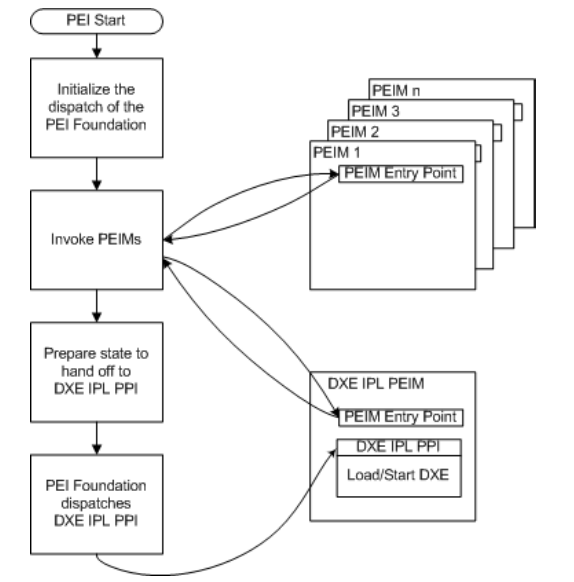
\includegraphics[width=0.8\linewidth]{design/pei-operation-diagram}
	\caption{Diagram of PI Operations}\label{fig:design-pei-operation-diagram}
\end{figure}

\subsubsection{PEI Services}
The PEI Foundation institutes a system table for the PEI Services named as PEI Services Table that is viewable to all \gls{pei} Modules (PEIMs) in the system. A PEI Service is defined as a method, command or other potentiality manifested by the PEI Foundation when that service's initialization needs are met. As the PEI phase having no permanent memory available until almost the end of the phase, all the various types of services created during this phase (PEI phase) cannot be as enrich as those created during later phases. A pointer to PEI Services Table is sent into entry point of each PEIM's and also to part of each PEIM-to-PEIM Interface (PPI) because the location of PEI Foundation and its temporary memory is unknown at build time. 

The PEI Foundation provides the classes of services listed in Table \ref{table:design-pei-foundation-class-service}

\begin{table}[h]
	\centering
	\renewcommand*{\arraystretch}{2}
	\caption{Services provided by PEI Foundation Classes}\label{table:design-pei-foundation-class-service}
	\begin{tabular}{ l | p{9cm} }
		Service & Details
		\\ \hline \hline
		PPI Services & Manages PPIs to ease inter-module method calls between PEIMs. A database maintained in temporary RAM to track installed interfaces.
		\\ \hline
		Boot Mode Services & Manages the boot mode (S3, S5, diagnostics, normal boot, etc.)
		\\ \hline
		HOB Services & Creates data structures (Hand-off-blocks) that are used to convey information to the next phase 
		\\ \hline
		Firmware Volume Services & Finds PEIMs and along with that other firmware files in the firmware volumes
		\\ \hline
		PEI Memory Services & provides a collection of memory management services (to be used before and after permanent memory to discovered)
		\\ \hline
		Status Code Services & Provides general progress and error code reporting services (i.e. port 080h or a serial port for text output for debug)
		\\ \hline
		Reset Services & Provides a common means to aid initializing warm or cold restart of the system
		\\ \hline
	\end{tabular}

\end{table}


\subsubsection{PEI Foundation}
The PEI Foundation is the entity that carried outs following activity:
\begin{itemize}
	\item Dispatching of Pre-EFI initialization modules (PEIMs)
	\item Maintaining the boot mode
	\item Initialization of permanent memory
	\item Invoking the DXE loader 
\end{itemize}
The PEI Foundation written to be portable across all the various platforms architecture of a given instruction-set. i.e. A binary for IA-32 (32-bit Intel architecture) works across all Pentium processors and similarly Itanium processor family work across all Itanium processors.

Irrespective of the processor micro architecture, the set of services uncovered by the PEI Foundation should be the same. This consistent surface area around the PEI Foundation allows PEIMs to be written in the \verb|C programming language| and compiled across any micro architecture.

\subsection{PEI Dispatcher}
The PEI Dispatcher is basically a state machine which is implemented in the PEI Foundation. The PEI Dispatcher evaluates the dependency expressions in Pre-EFI initialization modules (PEIMs) that are lying in the \gls{fv}s being examined.

Dependency expressions are coherent combinations of PEIM-to-PEIM Interfaces (PPIs). These expressions distinguish the PPIs that must be available for use before a given PEIM can be invoked. The PEI Dispatcher references the PPI database in the PEI Foundation to conclude which PPIs have to be installed and evaluate the dependency expression for the PEIM. If PPI has already been installed then dependency expression will evaluate to \verb|TRUE|, which notifies  PEI Dispatcher it can run PEIM. At this stage, the PEI Foundation handovers control to the PEIM with \verb|TRUE| dependency expression. 

The PEI Dispatcher will exit Once the PEI Dispatcher has examined and evaluated all of the PEIMs in all of the uncovered firmware volumes and no more PEIMs can be dispatched (i.e. the dependency expressions (\gls{depex}) do not evaluate from \verb|FALSE| to \verb|TRUE|). At this stage, the PEI Dispatcher cannot invoke any additional PEIMs. The PEI Foundation then takes back control from the PEI Dispatcher and calls the \verb|DXE IPL PPI| to navigate control to the DXE phase of execution.

\subsection{Drive Execution Environment (\gls{dxe})}
Before the DXE phase, the Pre-EFI Initialization (PEI) phase is held responsible for initializing permanent memory in the platform. Hence, DXE phase can be loaded and executed. At the very end of the PEI phase, state of the system is handed over to the DXE phase through Hand-Off Blocks (list of position independent data structures). 

There are three components in the DXE phase:
\begin{enumerate}
	\item DXE Foundation
	\item DXE Dispatcher
	\item A set of DXE Drivers
\end{enumerate}

\subsection{Boot Device Selection (\gls{bds})}
The BDS Architectural Protocol has part of implementation of the Boot Device Selection (BDS) phase. After evaluation of all of the DXE drivers dependencies, DXE drivers with satisfied dependencies are loaded and executed by the DXE Dispatcher, the DXE Foundation will pass the control to the BDS Architectural Protocol. The BDS phase held responsible for the following:

\begin{itemize}
	\item Initializing console devices
	\item Loading device drivers
	\item Attempt of loading and executing boot selections
\end{itemize}

\subsection{Transient System Load (TSL) and Runtime (RT)}
Primarily the OS vendor provides boot loader known as The Transient System Load (TSL). TSL and Runtime Services (RT) phases may allow access to persistent content, via UEFI drivers and applications. Drivers in this category include PCI Option ROMs.

\subsection{After Life (AL)}
The After Life (AL) phase contains the persistent UEFI drivers used to store the state of the system during the OS systematically shutdown, sleep, hibernate or restart processes.

